\input{../preamble.tex}
\def\arraystretch{1}
\setlength\tabcolsep{10pt}

\SetDate[20/03/2026]
\reversemarginpar
\setlength{\marginparsep}{.5cm}

\begin{document}
\pagestyle{fancy}
\fancyhead[L]{Seconde}
\fancyhead[C]{\textbf{Évaluation — Vecteurs}}
\fancyhead[R]{\today}

\null\vspace{-20pt}
Consignes particulières : 
\begin{itemize}[label=$\bullet$]
	\item 
	La calculatrice est {interdite}.
	\item
	Sauf mention du contraire, toutes les réponses doivent être justifiées.
	\item
	Les exercices \ref{exe:Chasles} et \ref{exe:det-area}.1 peuvent être entièrement faits sur la feuille d'évaluation.
	Noter son nom avant de rendre le sujet.
	\item
	L'évaluation fait \pageref{lastpage} page. La somme des points est \total{points}.
\end{itemize}

\marginpar{[pts]}
\hrule


\exe{4}{
	Considérons le point $A(0 ; -4)$, le vecteur $v = \pvec{1}{2}$, et la fonction $f(x) = 2x - 4$ \mbox{définie sur $\R$.}
	
	Posons $(d)$ la droite passant par $A$ et dirigée par $v$ et $\C_f$ la courbe représentative de $f$.
	
	\begin{enumerate}
		\item
		Donner un point $B$ différent de $A$ et appartenant à $(d)$.
		\item
		Est-ce que le point $B$ appartient à $\C_f$ ?
		\item
		Donner un point $C$ appartenant à $\C_f$ distinct des points déjà cités
		\item
		Est-ce que $C$ appartient à $(d)$ ?
	\end{enumerate}
}{exe:v-directeur}{
	
	\begin{enumerate}
		\item
		D'après le cours, $(d)$ est l'ensemble des translatés de $A$ par un multiple de $v$ :
			\[ (d) = \bigset{ A + k\cdot v \tq k \in \R}. \]
		En particulier, le point $A, B=A+v = (1 ; -2),$ appartient à $(d)$.
		
		\item
		D'après la propriété fondamentale, pour montrer que $B$ appartient à $\C_f$, il suffit de calculer $f(x_B)$ et de comparer avec $y_B$.
		Comme
			\begin{align*}
				f(x_B) &= f(1) = 2-4 = -2 = y_B,
			\end{align*}
		le point $B$ appartient à $\C_f$.
		
		\item
		Par définition, $\C_f$ est l'ensemble des points $\bigl(x ; f(x)\bigr)$ avec $x \in \R$.
		Prenons $x=7$ (notre nombre préféré) : le point $C(7 ; 10)$ appartient à $\C_f$.
		
		\item
		Pour montrer que $C$ appartient à $(d)$, il suffit de calculer $\vec{AC}$ et de montrer qu'il est colinéaire à $v$.
			\[ \vec{AC} = \pvec{7-0}{10-(-4)} = \pvec{7}{14} = 7u \]
	\end{enumerate}

}



\exe{4}{
	Pour chacune des propositions suivantes, \underline{justifier} qu'elle est toujours vraie à l'aide du cours ou \underline{dessiner} un contre-exemple.
	
	Soient $u, v, w$ trois vecteurs.
	\begin{enumerate}
		\item Si $v = -u$, alors $\det(u, v) = 0$.
		\item Si $\vec{AB}$ et $\vec{CD}$ sont colinéaires, alors les points $A, B, C$, et $D$ sont alignés.
		\item  Si $\norm{u} = \norm{v}$, alors $u$ et $v$ sont colinéaires.
		\item Si $u$ et $v$ sont colinéaires, alors $\norm{u} = \norm{v}$.
	\end{enumerate}
}{exe:QCM}{
	\begin{enumerate}
		\item 
		C'est vrai : si $v = -u$, les vecteurs sont colinéaires et donc leur déterminant est nul d'après le cours.
		
		Il est aussi possible de le montrer par le calcul :
			\[ \det\Bigl( \pvec{a}{b}, \pvec{-a}{-b} \Bigr) = (a)(-b) - (b)(-a) ) = -ab+ab = 0. \]
			
		\item 
		C'est faux en général : on sait que $(AB)$ et $(CD)$ sont parallèles, mais pas si les droites sont confondues.
		Un contre-exemple est donné par $A(0;0), B(1;0)$ et $C(1;0), D(1;1)$.
		
		\item 
		C'est faux : les deux vecteurs on la même norme (longueur de translation) mais pas nécessairement la même direction.
		Les vecteurs canoniques $\pvec10$ et $\pvec01$ donnent un contre-exemple naturel.
		
		\item 
		C'est faux : si deux vecteurs on la même direction, ils n'ont pas nécessairement la même norme (longueur de translation).
		Les vecteurs $\pvec10$ et $\pvec20$ forment un contre-exemple.
	\end{enumerate}
}


\exe{3}{
	Construire approximativement les vecteurs 
		\begin{align*}
			a = u+v, && b = -\frac{81}{40}w, && \text{ et } && c = 2u - \dfrac12v + \dfrac32w,
		\end{align*}
	où les vecteurs $u, v, w$ sont donnés dans le plan ci-dessous.
	Montrer les constructions.
	
	\begin{center}
		\begin{tikzpicture}[>=stealth, scale=1.2]
		\begin{axis}[xmin = -10, xmax=10, ymin=-10, ymax=10, axis x line=none, axis y line=none, axis line style=<->, xlabel={}, ylabel={}, ticks = none]
			\draw[very thick, ->, GREEN_E, xshift=-220, yshift=20] (axis cs:0,0) -- (axis cs: 4,-2) node[midway, above] {$u$};
			% u = (4, -2)
			\draw[very thick, ->, RED_E, xshift=-40, yshift=40] (axis cs: 0,0) -- (axis cs: -7,-6) node[midway, above] {$v$};
			% v = (-7, -6)
			\draw[very thick, ->, BLUE_E] (axis cs:0,0) -- (axis cs: -1,5) node[midway,right] {$w$};
			% w = (-1, 5)
		\end{axis}
		\end{tikzpicture}
	\end{center}
	%\vspace{-1cm}
	\underline{\textbf{Constructions :}}
	%\vspace{5cm}
}{exe:Chasles}{
	\begin{center}
		\begin{tikzpicture}[>=stealth, scale=1]
		\begin{axis}[xmin = -10, xmax=10, ymin=-10, ymax=10, axis x line=none, axis y line=none, axis line style=<->, xlabel={}, ylabel={}, ticks = none]
			\draw[very thick, ->, PINK, xshift=-120, yshift=60] (axis cs:0,0) -- (axis cs: -3,-8) node[midway, right] {$u+v$};
			% u = (4, -2)
			\draw[very thick, ->, GOLD_E, xshift=-40, yshift=60] (axis cs: 0,0) -- (axis cs: 81/40,-81/40*5) node[midway, left] {$-\frac{81}{40}w$};
			% v = (-7, -6)
			\draw[very thick, ->, TEAL_E, xshift=30, yshift=0] (axis cs:0,0) -- (axis cs: 8+7/2-3/2,-4+3+15/2) node[midway,below right] {$2u - \frac12v + \frac32w$};
			% w = (-1, 5)
		\end{axis}
		\end{tikzpicture}
	\end{center}
}

\newpage

\exe{10}{
	Considérons le point $A(-4; -2)$ et les deux vecteurs $u = \pvec{6}{2}$ et $v = \pvec{1}{-3}$.
	Posons de plus les trois points
		\begin{align*}
			B = A + u, && C = B + v, && D = C - u.
		\end{align*}
	Les questions $1$, $2$, et $3$ peuvent être faites séparément en admettant les résultats des questions précédentes.
	
	\begin{enumerate}
		\item 
		Montrer que $B(2;0), C(3;-3)$, et $D(-3;-5)$ puis dessiner le quadrilatère $ABCD$ dans le repère figure \ref{fig:1}.
		
		\item
		\begin{enumerate}[label=(\alph*)]
			\item Calculer les vecteurs $\vec{AB}$ et $\vec{DC}$ puis montrer qu'ils sont colinéaires.
			\item Calculer les vecteurs $\vec{AD}$ et $\vec{CB}$ puis montrer qu'ils sont colinéaires.
			\item Montrer que $\norm{\vec{AB}}= 2\sqrt{10}$, $\norm{\vec{AD}} = \sqrt{10}$, et $\norm{\vec{BD}} = 5\sqrt{2}$.
			\item Vérifier que $\det\Bigl(\vec{AB}, \vec{AD}\Bigr) = -20$.
		\end{enumerate}
		
		\item
		\begin{enumerate}[label=(\alph*)]
			\item Montrer que le quadrilatère $ABCD$ est un parallélogramme à l'aide des questions 2(a-b).
			
			%\emph{Un parallélogramme est un quadrilatère dont les côtés opposés sont parallèles.}
			\item Montrer que le triangle $ABD$ est rectangle en $A$ à l'aide de la réciproque du théorème de Pythagore et de la question 2(c).
			\item En déduire que $ABCD$ est un rectangle et calculer son aire à l'aide de la question 2(c).
			
			\emph{Aire d'un rectangle : (longueur) $\times$ (largeur).}
			\item Comparer l'aire obtenue à $\left| \det\Bigl(\vec{AB}, \vec{AD}\Bigr) \right|$, la valeur absolue du déterminant calculé à la question 2(d).
		\end{enumerate}
	\end{enumerate}
}{exe:det-area}{

	\begin{enumerate}
		\item 
		On calcule les coordonnées des points comme vu en classe.
			\begin{align*}
				B &= (-4 ; -2) + \pvec62 = (-4 + 6 ; -2+2) = (2 ; 0) \\
				C &= (2 ; 0) + \pvec1{-3} = (2+1 ; 0-3) = (3 ; -3) \\
				D &= (3 ; -3) - \pvec62 = (3-6 ; -3-2) = (-3 ; -5)
			\end{align*}
	\end{enumerate}
	
	\begin{center}
	\begin{tikzpicture}[>=stealth, scale=1]
		\begin{axis}[xmin = -5.5, xmax=5.5, ymin=-5.5, ymax=5.5, axis x line=middle, axis y line=middle, axis line style=<->, xlabel={}, ylabel={}, xtick distance=1, ytick distance=1, grid=both, x=1cm, y=1cm]
		\addplot[BLUE_E, mark=*] (-4,-2) node[above left]{$A$};
		\addplot[RED_E, mark=*] (2,0) node[above right]{$B$};
		\addplot[GREEN_E, mark=*] (3,-3) node[below right]{$C$};
		\addplot[GOLD_E, mark=*] (-3,-5) node[below left]{$D$};
		\addplot[GREY, dashed, thick] (-4,-2) -- (axis cs:2,0) -- (axis cs:3,-3) -- (axis cs:-3,-5) -- (axis cs:-4,-2);
		\end{axis}
	\end{tikzpicture}
	\end{center}
	\begin{enumerate}[resume]
		\item
		\begin{enumerate}[label=(\alph*)]
			\item 
			Comme $B = A + u = A + \vec{AB}$, on doit obtenir $\vec{AB} = u = \pvec62$.
			Comme $D = C-u = C + \vec{CD}$, on doit obtenir $\vec{CD} = -u = \pvec{-6}{-2}$.
			Ces deux vecteurs sont colinéaires car $-u = -1\times u$.
			\item
			Calculons
				\begin{align*}
					\vec{AD} &= \pvec{x_D - x_A}{y_D-y_A} = \pvec{-3-(-4)}{-5-(-2)} = \pvec{1}{-3}, \\
					\vec{CB} &= \pvec{x_B - x_C}{y_B-y_C} = \pvec{2-3}{0-(-3)} = \pvec{-1}{3}.
				\end{align*}
			Comme $\vec{AD} = -1\times\vec{CB}$, les deux vecteurs sont bien colinéaires.
			
			\item
			La formule de la norme $\norm{\pvec{x}{y}} = \sqrt{x^2 + y^2}$ permet de calculer les normes suivantes.
				\begin{align*}
					\norm{\vec{AB}} &= \sqrt{6^2 + 2^2} = \sqrt{40} = \sqrt4 \sqrt{10} = 2\sqrt10 \\
					\norm{\vec{AD}} &= \sqrt{1^2 + (-3)^2} = \sqrt{10} \\
					\norm{\vec{BD}} &= \norm{\pvec{-5}{5}} = \sqrt{(-5)^2 + 5^2} = \sqrt{50} = \sqrt{25}\sqrt2 = 5\sqrt2
				\end{align*}

			\item
			D'après la définition du déterminant, on obtient bien
				\[ \det\Bigl(\vec{AB}, \vec{AD}\Bigr) = \det\Bigl(\pvec62, \pvec1{-3}\Bigr) = (6)(-3)-(2)(1) = -18-2 = -20. \]
		\end{enumerate}
		
		\item
		\begin{enumerate}[label=(\alph*)]
			\item 
			Les droites $(AB)$ et $(CD)$ sont parallèles d'après la question 2(a) et les droites $(AD)$ et $(BC)$ sont parallèles d'après la question 2(b) : le quadrilatère est un parallélogramme.
			\item
			Il s'agit de montrer l'identité $BD^2 \stackrel{?}{=} AB^2 + AD^2$.
			
			À gauche, $BD^2 = \norm{\vec{BD}}^2 = \left(5\sqrt2\right)^2 = 25\times2 = 50$.
			
			À droite, $AB^2 + AD^2 = \left(2\sqrt{10}\right)^2 + \sqrt{10}^2 = 4\times10 + 10 = 50$.
			
			L'identité est donc vraie et la réciproque du théorème de Pythagore conclut : le triangle $ABD$ est rectangle en $A$.
			
			\item
			Le quadrilatère $ABCD$ est un parallélogramme qui admet un angle droit : c'est nécessairement un rectangle car ses côtés sont perpendiculaires deux à deux par parallélisme.
			
			Par conséquent, l'aire est donnée par $AB \times AD = 2 \sqrt{10} \times \sqrt{10} = 2 \times 10 = 20$.
			
			\item
			La valeur absolue du déterminant est $\abs{-20} = 20$, égale à l'aire du rectangle.
		\end{enumerate}
	\end{enumerate}



}

\begin{figure}[h!]
	
	\begin{center}
	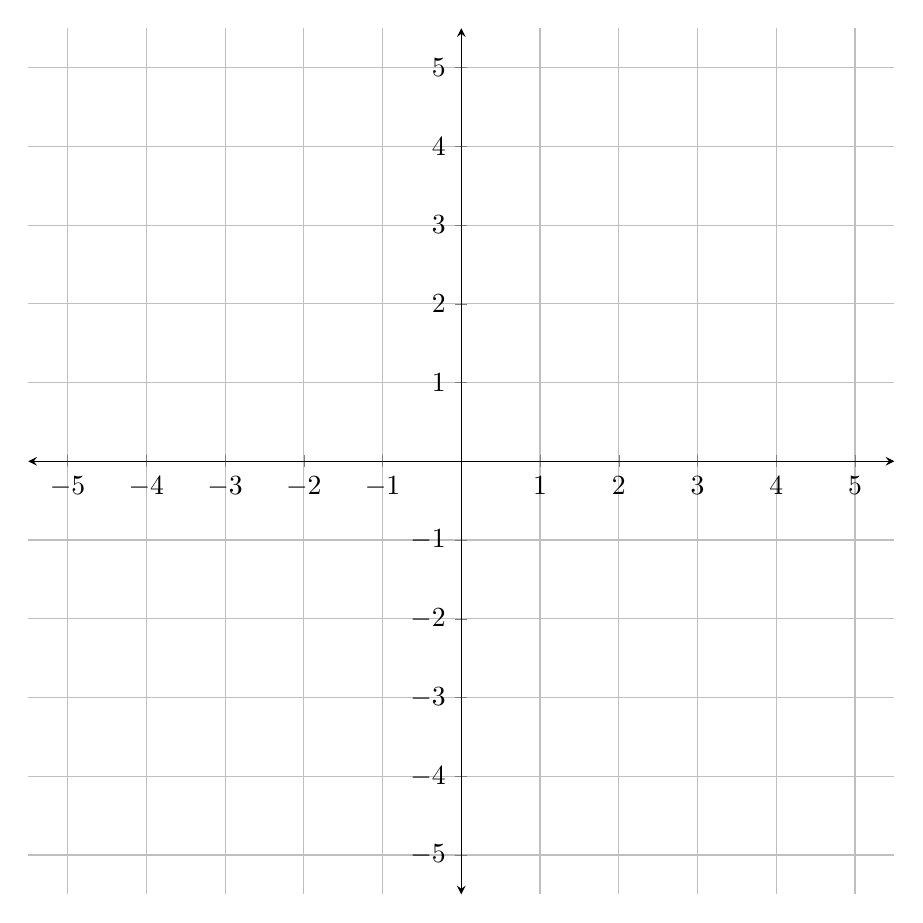
\begin{tikzpicture}[>=stealth, scale=1]
		\begin{axis}[xmin = -5.5, xmax=5.5, ymin=-5.5, ymax=5.5, axis x line=middle, axis y line=middle, axis line style=<->, xlabel={}, ylabel={}, xtick distance=1, ytick distance=1, grid=both, x=1cm, y=1cm]
		\end{axis}
	\end{tikzpicture}
	\end{center}
	
	\caption{Repère de l'exercice \ref{exe:det-area}.}
	\label{fig:1}

\end{figure}

%%%%%%%%%%%

\label{lastpage}
\newpage
\fancyhead[C]{\textbf{Solutions}}
\shipoutAnswer
	
\end{document}
